%%%%%%%%%%%%%%%%%%%%%%%%%%%%%%%%%%%%%%%%%
% University/School Laboratory Report
% LaTeX Template
% Version 3.1 (25/3/14)
%
% This template has been downloaded from:
% http://www.LaTeXTemplates.com
%
% Original author:
% Linux and Unix Users Group at Virginia Tech Wiki 
% (https://vtluug.org/wiki/Example_LaTeX_chem_lab_report)
%
% License:
% CC BY-NC-SA 3.0 (http://creativecommons.org/licenses/by-nc-sa/3.0/)
%
%%%%%%%%%%%%%%%%%%%%%%%%%%%%%%%%%%%%%%%%%

%----------------------------------------------------------------------------------------
%	PACKAGES AND DOCUMENT CONFIGURATIONS
%----------------------------------------------------------------------------------------
\documentclass{article}

%\usepackage[version=3]{mhchem} % Package for chemical equation typesetting
\usepackage{siunitx} % Provides the \SI{}{} and \si{} command for typesetting SI units
\usepackage{graphicx} % Required for the inclusion of images
\usepackage{natbib} % Required to change bibliography style to APA
\usepackage{amsmath} % Required for some math elements 
\usepackage{framed, color}

\setlength\parindent{0pt} % Removes all indentation from paragraphs

\renewcommand{\labelenumi}{\alph{enumi}.} % Make numbering in the enumerate environment by letter rather than number (e.g. section 6)

%\usepackage{times} % Uncomment to use the Times New Roman font

%----------------------------------------------------------------------------------------
%	DOCUMENT INFORMATION
%----------------------------------------------------------------------------------------
\title{Regelung eines Furuta Pendulums} % Title

\author{
Thomas \textsc{Schildhauer} \\
Dustin \textsc{Horenburg} \\
Kai \textsc{Hamann} } % Author name


\date{\today} % Date for the report

\begin{document}

\maketitle % Insert the title, author and date

\vspace{2cm}

\begin{center}
%\begin{tabular}{l r}
Mechatronics Lab \\
Sommersemester 2015 \\ 
Betreuer: Dipl.-Ing. Martin Gomse
%\end{tabular}

\vspace{2cm}

\begin{tabular}{l c r}
Thomas Schildhauer	& MEC & 21156392 \\
Dustin Horenburg	& MEC & 21153749 \\
Kai Hamann			& MEC & 21156059

\end{tabular}
\end{center}

% If you wish to include an abstract, uncomment the lines below
% \begin{abstract}
% Abstract text
% \end{abstract}

\tableofcontents
%----------------------------------------------------------------------------------------
%	SECTION 1
%----------------------------------------------------------------------------------------
\section{Einleitung}
\label{sec.Einleitung}

Dieser Bericht befasst sich mit der Modellierung und der Regelung eines invertierten Pendels, das auch \emph{Furuta-Pendel} genannt wird. 
Ziel des Labors ist es, einen robusten Regler zu entwerfen der die folgenden drei Aufgaben erfüllt:
\begin{enumerate}
	\raggedright
	\item Das Pendel aufschwingen, bis der \emph{Schwingarm} durch die grenzstabile aufrechte Lage schwingt.
	\item Den \emph{Schwingarm} in der aufrechten Lage fangen und dort halten.
	\item Den \emph{Dreharm} zurück zur Ausgangslage bringen, ohne dass dabei der \emph{Schwingarm} aus der aufrechten Lage herausfällt.
\end{enumerate}
Im folgenden Bericht wird der \emph{Dreharm} mit Arm~1 und der \emph{Schwingarm} mit Arm~2 bezeichnet.
Für weitere Erläuterungen sei auf Abschnitt~\ref{sec.Theorie} verwiesen.
Der Bericht ist Teil des Fachlabors Mechatronik im Sommersemester 2015 an der Technischen Universität Hamburg-Harburg und stellt die im Zuge dieses Labors durchgeführten Berechnungen, Modellierungen und Versuche dar. 
Für die mathematische Modellierung und die Auslegung der Regler werden Matlab und Simulink verwendet.
Diese Programme stehen den Autoren von der Universität aus zur Verfügung.

Abschnitt~\ref{sec.Theorie} befasst sich mit den nötigen theoretischen Grundlagen und der mathematischen Modellierung des Pendels.
Dort wird primär auf die Quelle~\citep{Cazzolato.2011} eingegangen, welche als Vorlage genutzt wurde und vom Betreuer des Labors zur Verfügung gestellt wurde.

In Abschnitt~\ref{sec.Parameter} werden die für die Regelung nötigen Parameter aus dem realen Pendel abgeleitet. 
Gemessene Größen wie Massen und Längen des realen Pendels werden dazu umgeformt und zusammengefasst, um diese auf die Form des mathematischen Modells zu bringen.
Es folgt eine Auflistung der auf diese Weise identifizierten Größen, die in das mathematische Modell einfließen und die Grundlage für die Regelung bilden.

Die Auslegung und Implementierung der Regler in Matlab und Simulink wird in Abschnitt~\ref{sec.Controller} behandelt.
Es wird auf die verschiedenen Formen von Regelungsalgorithmen eingegangen, die eingesetzt werden, um die oben beschriebenen Anforderungen zu erfüllen, und darauf, wie zwischen diesen je nach Zustand des Pendels gewechselt werden kann.
Außerdem wird ein Algorithmus zur Unterscheidung zweier unterschiedlicher Pendelarme ausgelegt. 
Es soll damit möglich sein, automatisch zu identifizieren, welcher der beiden vorgegebenen Pendelarme aktuell montiert ist. 
Die Pendelarme unterscheiden sich in Masse und Stablänge.

Ergebnisse verschiedener Messungen an dem realen Furuta-Pendel werden in Abschnitt~\ref{sec.Ergebnisse} präsentiert. 
Dort finden sich verschiedene Versuche zum Testen der Funktion und der Robustheit des Reglers.
Es werden jeweils Messergebnisse präsentiert, welche die Funktionalität der verschiedenen Regelungsalgorithmen und deren Zusammenspiel verdeutlichen sollen.

Im letzten Abschnitt folgen Fazit und Ausblick, in denen auf die wesentlichen Erkenntnisse dieses Laborprojekts noch einmal eingegangen wird.


%----------------------------------------------------------------------------------------
%	SECTION 2
%----------------------------------------------------------------------------------------
\section{Theorie}
\label{sec.Theorie}
In diesem Abschnitt wird auf die Theorie des sogenannten \emph{Furuta Pendels} eingegangen. Zunächst wird ein Modell des Pendels beschrieben. Im Anschluss wird die Theorie dieses Modells auf ein echtes Furuta Pendel angewandt. %Thomas: Diesen Text überarbeiten wenn der Abschnitt fertig ist.

\subsection{Furuta Pendel}
\label{sub.Furuta-Pendel}
Bei dem \emph{Furuta Pendel}, auch drehbares invertiertes Pendel genannt, handelt es sich um ein 1992 von Katsuhisa Furuta entwickeltes mechanisches Pendel. 
Es besteht aus einem angetriebenen Arm, welcher in der horizontalen Ebene rotieren kann. 
An diesem Arm ist ein Pendelarm befestigt, welcher frei in der zum angetriebenen Arm orthogonalen Ebene rotiert. 
Das Furuta Pendel ist ein Beispiel eines komplexen nichtlinearen Oszillators. \citep{Cazzolato.2011}

\begin{figure}[htbp]
	\centering
	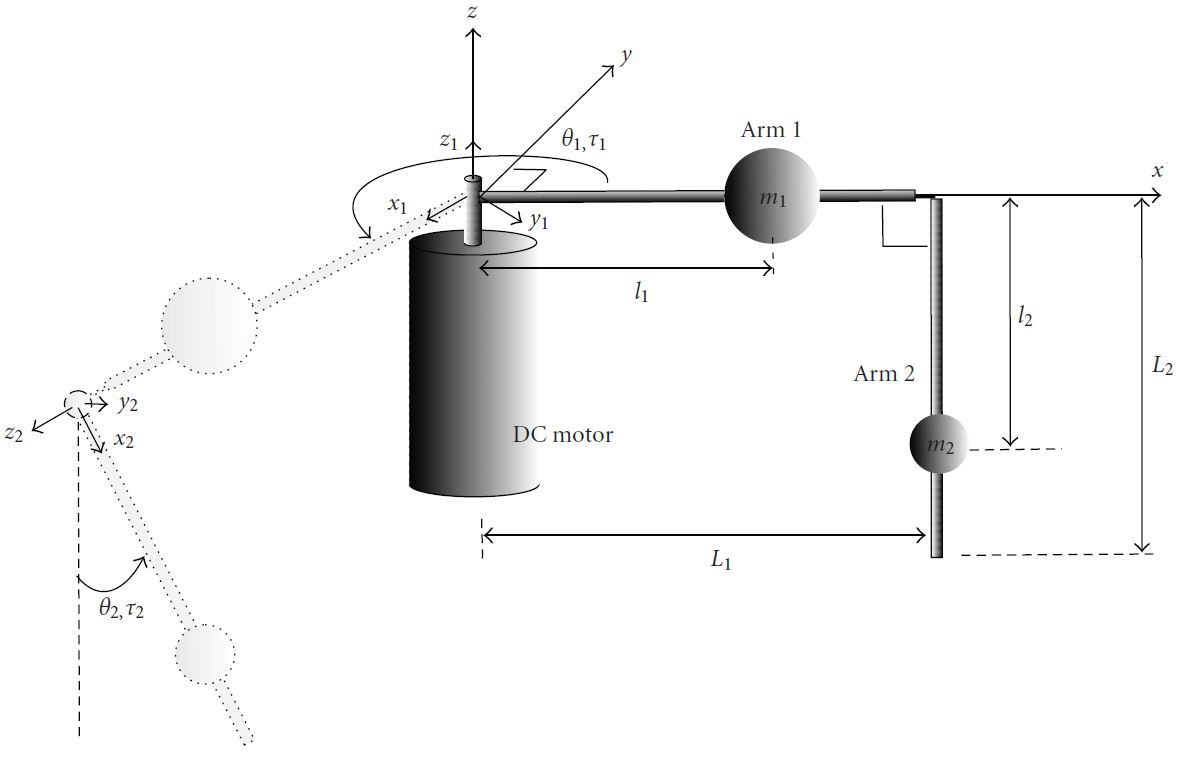
\includegraphics[width=1.\textwidth]{Grafiken/furuta3.jpg}
	\caption{Furuta Pendel nach~\cite{Cazzolato.2011}. }
	\label{fig.furuta-schematic}
\end{figure}

Abbildung~\ref{fig.furuta-schematic} zeigt das Schema eines Furuta Pendels, welches von einem DC-Elektromotor angetrieben wird.
Mit dem Motor wird ein Drehmoment $\tau_1$ auf Arm~1 des Pendels gebracht. 
Das Drehmoment $\tau_2$ bezeichnet das Kopplungsmoment zwischen Arm~1 und Arm~2. 
Die Verbindung zwischen Arm~1 und Arm~2 rotiert frei und ist nicht angetrieben.
Die beiden Arme haben die Längen $L_1$ und $L_2$ sowie die Massen $m_1$ und $m_2$.
$l_1$ und $l_2$ bezeichnen die jeweiligen Abstände der Massenmittelpunkte zum Rotationspunkt der Arme.
Die Arme besitzen die Trägheitstensoren $J_1$ und $J_2$ um ihren jeweiligen Massenmittelpunkt und ihre Gelenke unterliegen linearer Dämpfung mit den Dämpfungskonstanten $b_1$ und~$b_2$.

\subsection{Annahmen}
\label{sub.sub.Annahmen}
Vor der Aufstellung des Gleichungssystems werden in~\cite{Cazzolato.2011} einige Annahmen getroffen, die an dieser Stelle kurz wiederholt werden:
\begin{enumerate}
\item Die Kopplung zwischen Motorachse und Arm~1 wird als ideal starr angenommen.
\item Die Motorachse und beide Pendelarme werden als ideal starr angenommen.
\item Die Koordinatensysteme von Arm~1 und Arm~2 sind die Hauptachsensysteme, sodass die Trägheitstensoren diagonal sind.
\item Die Trägheit des Motors wird vernachlässigt. %Thomas: trifft das auf uns zu????
\item Es wird von reiner linearer (viskoser) Dämpfung ausgegangen.
\end{enumerate}

\subsection{Mathematisches Modell}
\label{sub.sub.Mathematisches-Modell}
Mit den in Abschnitt~\ref{sub.sub.Annahmen} getroffenen Annahmen wird in~\cite{Cazzolato.2011} ein mathematisches Modell entwickelt, mit dem die Winkelbeschleunigung der beiden Pendelarme in Abhängigkeit der Zustands\-varibalen beschrieben werden kann. 
Zunächst wird die Gleichung für die beiden Drehmomente $\tau_1$ und $\tau_2$ in Abhängigkeit der Trägheitstensoren $J_1$ und $J_2$ aufgestellt.
(Für nähre Ausführungen sei auf~\cite{Cazzolato.2011} verwiesen.)

\begin{equation}
\label{eqn.TauComplex}
\begin{bmatrix}
\tau_1 \\
\tau_2
\end{bmatrix}
=
\begin{bmatrix}
\begin{pmatrix}
\ddot{\theta}_1(J_{1zz}+m_1l^2_1+m_2L^2_1+(J_{2yy}+m_2l^2_2) 						\\
\times \sin^2(\theta_2)+J_{2xx}cos^2(\theta_2))+\ddot{\theta}_2m_2L_1l_2\cos(\theta_2)			\\
-m_2L_1l_2\sin(\theta_2)\dot{\theta}^2_2+\dot{\theta}_1\dot{\theta}_2\sin(2\theta_2)	\\
\times(m_2l^2_2+J_{2yy}-J_{2xx})+b_1\dot{\theta}_1
\end{pmatrix}
\\
\begin{pmatrix}
\ddot{\theta}_1m_2L_1l_2\cos(\theta_2)+\ddot{\theta}_2(m_2l^2_2+J_{2zz})	\\
+\frac{1}{2}\dot{\theta}_1\sin(2\theta_2)(-m_2l^2_2-J_{2yy}+J_{2xx})						\\
+b_2\dot{\theta}_2+gm_2l_2\sin(\theta_2)
\end{pmatrix}
\end{bmatrix}
\end{equation}

Die Trägheitstensoren der beiden Pendelarme können nun unter den Annahmen $J_{xx} \approx 0$ und $J_{yy} \approx J_{zz}$ wie folgt vereinfacht werden: 
\begin{align}
\label{eqn.Tragheitstensoren}
J_1&=
\begin{bmatrix}
J_{1xx} & 0 & 0\\
0 & J_{1yy} & 0\\
0 & 0 & J_{1zz}
\end{bmatrix}
&\approx
\begin{bmatrix}
0 & 0 & 0\\
0 & \bar{J}_{1} & 0\\
0 & 0 & \bar{J}_{1}
\end{bmatrix}
\nonumber \\
J_2&=
\begin{bmatrix}
J_{2xx} & 0 & 0\\
0 & J_{2yy} & 0\\
0 & 0 & J_{2zz}
\end{bmatrix}
&\approx
\begin{bmatrix}
0 & 0 & 0\\
0 & \bar{J}_{2} & 0\\
0 & 0 & \bar{J}_{2}
\end{bmatrix}
\end{align}

Folgende Bezeichnungen werden zur Vereinfachung von Gleichung~\ref{eqn.TauComplex} eingeführt.
\begin{eqnarray}
\hat{J}_1 &=& \bar{J}_1 + m_1l^2_1	\nonumber	\\
\hat{J}_2 &=& \bar{J}_2 + m_2l^2_2	\nonumber	\\
\hat{J}_0 &=& \bar{J}_1 + m_1l^2_1 + m_2L^2_1
\end{eqnarray}

So lassen sich die Formeln für die beiden Drehmomente $\tau_1$ und $\tau_2$ darstellen als:
\begin{equation}
\begin{bmatrix}
\tau_1 \\
\tau_2
\end{bmatrix}
=
\begin{bmatrix}
\begin{pmatrix}
\ddot{\theta}_1(\hat{J}_0+\hat{J}_2\sin^2(\theta_2))+\ddot{\theta}_2m_2L_1l_2\cos(\theta_2)			\\
-m_2L_1l_2\sin(\theta_2)\dot{\theta}^2_2+\dot{\theta}_1\dot{\theta}_2\hat{J}_2\sin(2\theta_2)+b_1\dot{\theta}_1
\end{pmatrix}
\\
\begin{pmatrix}
\ddot{\theta}_1m_2L_1l_2\cos(\theta_2)+\ddot{\theta}_2\hat{J}_2-\frac{1}{2}\dot{\theta}^2_1\hat{J}_2\sin(2\theta_2)						\\
+b_2\dot{\theta}_2+gm_2l_2\sin(\theta_2)
\end{pmatrix}
\end{bmatrix}
\end{equation}

Hieraus ergeben sich die folgenden nichtlinearen Differentialgleichungen für die Bewegung des Pendels. 
In~\cite{Cazzolato.2011} wird bei der Aufstellung dieser ein Vorzeichenfehler gemacht, der an dieser Stelle korrigiert ist und auf den nicht näher eingegangen wird.


%\colorbox{yellow}{Die folgenden Gleichungen enthalten noch den Fehler, den wir finden sollten.} \\
%\colorbox{yellow}{Ich habe die Lösung gerade nicht parat.Thomas: ich auch noch nicht}
Nachfolgend die nichtlinearen Differentialgleichungen für die Winkelbeschleunigung von Arm~1;
\begin{multline}
\ddot{\theta}_1 =
\frac{
\begin{bmatrix}
	-\hat{J}_2b_1 \\ 
	m_2L_1l_2\cos(\theta_2)b_2 \\ 
	-\hat{J}^2_2\sin(2\theta_2) \\ 
	-\frac{1}{2}\hat{J}_2m_2L_1l_2\cos(\theta_2)\sin(2\theta_2) \\ 
	\hat{J}_2m_2L_1l_2\sin(\theta_2)
\end{bmatrix}^T
\begin{bmatrix}
	\dot{\theta}_1 \\ 
	\dot{\theta}_2 \\ 
	\dot{\theta}_1\dot{\theta}_2 \\ 
	\dot{\theta}^2_1 \\ 
	\dot{\theta}^2_2
\end{bmatrix} }
{\hat{J}_0\hat{J}_2+\hat{J}^2_2\sin^2(\theta_2)-m^2_2L^2_1l^2_2\cos^2(\theta_2)} \\ 
%<--linebreak here
+
\frac{
\begin{bmatrix}
	\hat{J}_2 \\ 
	-m_2L_1l_2\cos(\theta_2) \\ 
	\frac{1}{2}m^2_2l^2_2L_1\sin(2\theta_2)
\end{bmatrix}^T
\begin{bmatrix}
	\tau_1 \\ 
	\tau_2 \\ 
	g
\end{bmatrix} }
{\hat{J}_0\hat{J}_2+\hat{J}^2_2\sin^2(\theta_2)-m^2_2L^2_1l^2_2\cos^2(\theta_2)}
\end{multline}

und die Winkelbeschleunigung von Arm~2:

\begin{multline}
\ddot{\theta}_2 =
\frac{
\begin{bmatrix}
	m_2L_1l_2\cos(\theta_2)b_1 \\ 
	-b_2(\hat{J}_0+\hat{J}_2\sin^2(\theta_2)) \\ 
	m_2L_1l_2\hat{J}_2\cos(\theta_2)\sin(2\theta_2) \\ 
	\frac{1}{2}\sin(2\theta_2)(\hat{J}_0\hat{J}_2+\hat{J}^2_2\sin^2(\theta_2)) \\ 
	-\frac{1}{2}m^2_2L^2_1l^2_2\sin(2\theta_2)
\end{bmatrix}^T
\begin{bmatrix}
	\dot{\theta}_1 \\ 
	\dot{\theta}_2 \\ 
	\dot{\theta}_1\dot{\theta}_2 \\ 
	\dot{\theta}^2_1 \\ 
	\dot{\theta}^2_2
\end{bmatrix} }
{\hat{J}_0\hat{J}_2+\hat{J}^2_2\sin^2(\theta_2)-m^2_2L^2_1l^2_2\cos^2(\theta_2)} \\
%<--linebreak here
+
\frac{
\begin{bmatrix}
	-m_2l_2\cos(\theta_2) \\ 
	\hat{J}_0+\hat{J}_2\sin^2(\theta_2) \\ 
	-m_2l_2\sin(\theta_2)(\hat{J}_0+\hat{J}_2\sin^2(\theta_2))
\end{bmatrix}^T
\begin{bmatrix}
	\tau_1 \\ 
	\tau_2 \\ 
	g
\end{bmatrix} }
{\hat{J}_0\hat{J}_2+\hat{J}^2_2\sin^2(\theta_2)-m^2_2L^2_1l^2_2\cos^2(\theta_2)}
\end{multline}

Diese entsprechen den Gleichungen~(33) und~(34) in~\cite{Cazzolato.2011}.

\subsection{Linearisierung}
\label{sub.sub.Linearisierung}
Die korrigierten nichtlinearen Differentialgleichungen aus Abschnitt~\ref{sub.sub.Mathematisches-Modell} werden in diesem Abschnitt nach dem Vorbild von~\cite{Cazzolato.2011} für den grenz\-stabilen oberen Gleichgewichtszustand ($\theta_2 = \pi$) linearisiert.

So ergeben sich folgende Zustands-Variablen für den Gleichgewichtszustand:
\begin{eqnarray}
\theta_{1e} &=& 0		\nonumber \\
\theta_{2e} &=& \pi	\nonumber \\
\dot{\theta}_{1e} &=& 0		\nonumber \\
\dot{\theta}_{2e} &=& 0	
\end{eqnarray}

Nach dem Vorbild von~\cite{Cazzolato.2011} kann so ein lineares Differentialgleichungssystem erster Ordnung aufgestellt werden. 
Ein solches System ist notwendig, um gängige Theorien für den Entwurf von Reglern zu nutzen~\citep{Werner.2013}. 
\begin{equation}
\begin{bmatrix}
\dot{\theta}_1 \\ 
\dot{\theta}_2 \\ 
\ddot{\theta}_1 \\ 
\ddot{\theta}_2
\end{bmatrix}
=
\begin{bmatrix}
0 & 0 & 1 & 0 \\ 
0 & 0 & 0 & 1 \\ 
A_{31} & A_{32} & A_{33} & A_{34} \\ 
A_{41} & A_{42} & A_{43} & A_{44}
\end{bmatrix}
\begin{bmatrix}
\theta_1 \\ 
\theta_2 \\ 
\dot{\theta}_1 \\
\dot{\theta}_2
\end{bmatrix}
+
\begin{bmatrix}
0 & 0 \\ 
0 & 0 \\ 
B_{31} & B_{32} \\ 
B_{41} & B_{42}
\end{bmatrix}
\begin{bmatrix}
\tau_1 \\ 
\tau_2
\end{bmatrix}
\end{equation}

Nach dem Einsetzen der Zustands-Variablen im Gleichgewichtszustand erhalten wir die Matrixeinträge in Abhängigkeit der Variablen aus Abschnitt~\ref{sub.sub.Mathematisches-Modell}.
\begin{eqnarray}
A_{31} &=& 0	\nonumber \\
A_{32} &=& \frac{gm^2_2l^2_2L_1}{(\hat{J}_0\hat{J}_2-m^2_2L^2_1l^2_2)}	\nonumber \\
A_{33} &=& \frac{-b_1\hat{J}_2}{(\hat{J}_0\hat{J}_2-m^2_2L^2_1l^2_2)}	\nonumber \\
A_{34} &=& \frac{-b_2m_2l_2L_1}{(\hat{J}_0\hat{J}_2-m^2_2L^2_1l^2_2)}	\nonumber \\
A_{41} &=& 0	\nonumber \\
A_{42} &=& \frac{gm_2l_2\hat{J}_0}{(\hat{J}_0\hat{J}_2-m^2_2L^2_1l^2_2)}	\nonumber \\
A_{43} &=& \frac{-b_1m_2l_2L_1}{(\hat{J}_0\hat{J}_2-m^2_2L^2_1l^2_2)}	\nonumber \\
A_{44} &=& \frac{-b_2\hat{J}_0}{(\hat{J}_0\hat{J}_2-m^2_2L^2_1l^2_2)}	\nonumber \\
\end{eqnarray}
\begin{eqnarray}
B_{31} &=& \frac{\hat{J}_2}{(\hat{J}_0\hat{J}_2-m^2_2L^2_1l^2_2)}	\nonumber \\
B_{41} &=& \frac{m_2L_1l_2}{(\hat{J}_0\hat{J}_2-m^2_2L^2_1l^2_2)}	\nonumber \\
B_{32} &=& \frac{m_2L_1l_2}{(\hat{J}_0\hat{J}_2-m^2_2L^2_1l^2_2)}	\nonumber \\
B_{42} &=& \frac{\hat{J}_0}{(\hat{J}_0\hat{J}_2-m^2_2L^2_1l^2_2)}	\nonumber \\
\end{eqnarray}


%----------------------------------------------------------------------------------------
%	SECTION 3
%----------------------------------------------------------------------------------------
\section{Identifikation der Parameter}
\label{sec.Parameter}
Das im Theorieteil betrachtete Modell des Furuta-Pendels (siehe \cite{Cazzolato.2011}) unterscheidet sich von dem Modell des zu verwendenden Furuta-Pendels des Institutes, wie in Abbildung~\ref{fig.FurutaPlant} ersichtlich.

\begin{figure}[htbp]
	\centering
	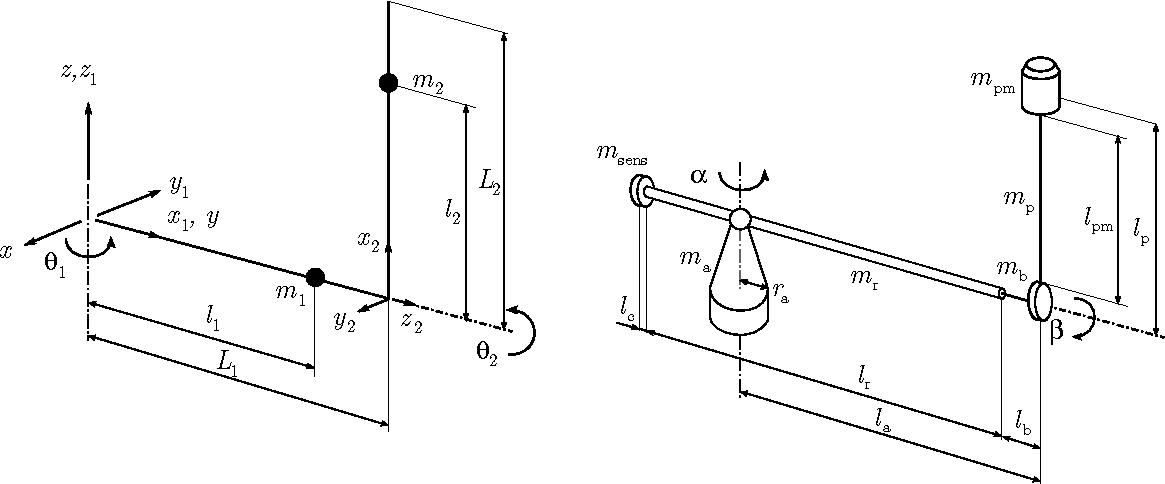
\includegraphics[width=1.\textwidth]{Grafiken/adelaideimagenew}
	\caption{Darstellung des Furuta-Pendels. (Zur Verfügung gestellt vom Betreuer des Labors) }
	\label{fig.FurutaPlant}
\end{figure}

Die gegeben bzw. gemessenen Parameter müssen daher an das theoretische Modell angepasst werden. Für die Längen der Pendelarme gilt somit:
\begin{eqnarray}
L_1 &=& l_a \nonumber \\
L_2 &=& l_{pm} \nonumber \\
l_{sens}=l_r+l_b-l_a+\dfrac{l_c2}{2}
\end{eqnarray}


Die Punktmassen des theoretischen Pendel-Modells ergeben sich bei Beachtung der Trägheitsachsen zu:
\begin{eqnarray}
m_1 &=& m_{sens}+m_r+m_a \nonumber \\
m_2 &=& m_p+m_{pm}
\end{eqnarray}
Die Massenträgheiten können ebenso zusammengefasst werden und ergeben sich wie folgt:
%Kai: ich habe einfach unsere equations aus matlab eingefügt!
%Thomas: ja, das merkt man ^^ hier ist gan
\begin{eqnarray*}
J_{1,norm}&=&\dfrac{J_M +J_{Enc,1}+(m_r \cdot l_r \cdot l_r)}{12+(m_r (-0.5 l_r-l_b+l_a)^2)+(\dfrac{4}{10}) (m_a  {r_a}^{2})} \\
J_{2,norm}&=& J_{m,b}+J_{Enc2}   + \dfrac{(m_p \cdot {l_p}^{2})}{3} \\
J_0&=&J_{1,norm}+ m_1 \cdot {l_1}^{2} + m_2 \cdot {L_1}^{2} \\ 
J_2&=&J_{2,norm}+m_2 \cdot {l_2}^2           \\
\end{eqnarray*}
Für die Längen $l_1$ und $l_2$ erhält man
\begin{align*}
l_1 &= \sqrt{\frac{(l_{sens}^2 \dot m_{sens}+l_b^2 \dot m_b)}{m_{sens} + m_b})} \\
l_2 &\cong l_{pm}
\end{align*}

%Kai: ab hier sind das wieder die von dustin/den anderen!
und für die einzelnen Trägheitsmomente:
\begin{align*}
J_{arm} &= m_r \frac{l^2_r}{12}+m_r(\frac{1}{2}l_r+l_b-l_a)^2 \\
J_{pend,1} &= m_bl^2_a \\
J_{sens} &= m_{sens}(l_a-l_b-l_r-\frac{1}{2}l_c)^2 \\
J_{ps} &= m_p(r_b+\frac{1}{2}l_p)^2 \\
J_{pm} &= m_{pm}l^2_{pm} \\
J_{arm}+J_{pend1}+J_{sens} &= m_1l^2_1 \\ 
J_{pm}+J_{ps} &= m_2l^2_2 \\
\end{align*}

%Hier sind unsere werte! noch viele Latex-Fehler!
% Thomas: ich schreib hier mal einen Absatz.
Die folgenden Werte sind im Zuge des Labors zu Verfügung gestellt oder durch rudimentäre Messungen erhalten und werden an dieser Stelle der Vollständigkeit halber aufgeführt. 
\begin{align*}
b_1 &= \SI{1e-4}{\newton\metre\second} &
b_2 &= \SI{2.8e-4}{\newton\metre\second} \\
g &= \SI{9.81}{\metre\per\square\second} &
k_{1,phi} &= \SI{0.5}{}\\
R_a &= \SI{10}{\ohm} &
J_M  &=  \SI{6.75e-6}{\kilo\gram\square\metre}  \\        % Inertia Motor 6.75e-6
J_{Enc1}  &=  \SI{6e-14}{\kilo\gram\square\metre}  &        % Inertia Encoder Theta1
J_{Enc2}  &=  \SI{0.1e-6}{\kilo\gram\square\metre}  \\     % Inertia Encoder Theta2
J_{m,b}  &=  \SI{3.98125e-6}{\kilo\gram\square\metre}  &     % Inertia m_b
m_{sens}  &=  \SI{0.084}{\kilo\gram}  \\
l_c  &=  \SI{0.01}{\metre}  &
m_{horzArm} &= \SI{0.284}{\metre} \\
m_b &= \SI{0.025}{\metre}  &
m_a &= \SI{0.190}{\metre} \\
r_a &= \SI{0.015}{\metre}  &
r_b &= \SI{0.0176}{\metre} \\
l_r &= \SI{0.29}{\metre} &
m_r  &=  m_{horzArm} - m_{sens}\\
l_a &= \SI{.175}{\metre} &
l_b &= \SI{.01}{\metre}\\
m_{pm} &= \SI{0.0379}{\kilo\gram} &
m_p &= \SI{0.0157}{\kilo\gram}\\
l_{pm} &= \SI{0.229}{\metre} &
l_p &= \SI{0.262}{\metre}\\
\end{align*}


Die Gleichung des DC-Motors, der den Pendelarm und somit direkt $\theta_2$ antreibt, kann aus der gegebenen Formel des Research Articles der University of Adelaide, abgeleitet werden.\cite{Cazzolato.2011}
Auch die Parameter des DC-Motors wurden aus dem Dokument entnommen. Folgende Parameter sind gegeben:

\begin{align}
K_m &= 0,09  \dfrac{Nm}{A} \\
R_m &= 7,8  \Omega \\
L_m &= 0,005  H 
\end{align}
%----------------------------------------------------------------------------------------
%	SECTION 4
%----------------------------------------------------------------------------------------
\section{Design der Controller}
\label{sec.Controller}
\subsection{Pendelidentifikation}
\label{Pendelidentifikation}
Beim Starten des Programmes zur Regelung des Pendels wird zunächst identifiziert, um welchen Pendelaufbau es sich handelt. Es wird dabei zwischen zwei zuvor definierten Pendelkonfigurationen unterschieden.
Für die Identifikation wird, nach einem kurzen Impuls durch den Motor, das Pendel frei schwingen gelassen, während der Controller den Verlauf von~$\theta_2$ aufzeichnet. Im Anschluss daran ist es möglich, aus den erhobenen Daten die Frequenz von~$\theta_2$ zu berechnen. Da sich die Frequenzen der Pendelkonfigurationen unterscheiden, kann das Programm so die entsprechenden Modelldaten laden und für die Regelung verwenden. In Abbildung \ref{fig.Identifikation} ist dieser Vorgang in den ersten fünf Sekunden zu erkennen.

\begin{figure}[htbp]
	\centering	
	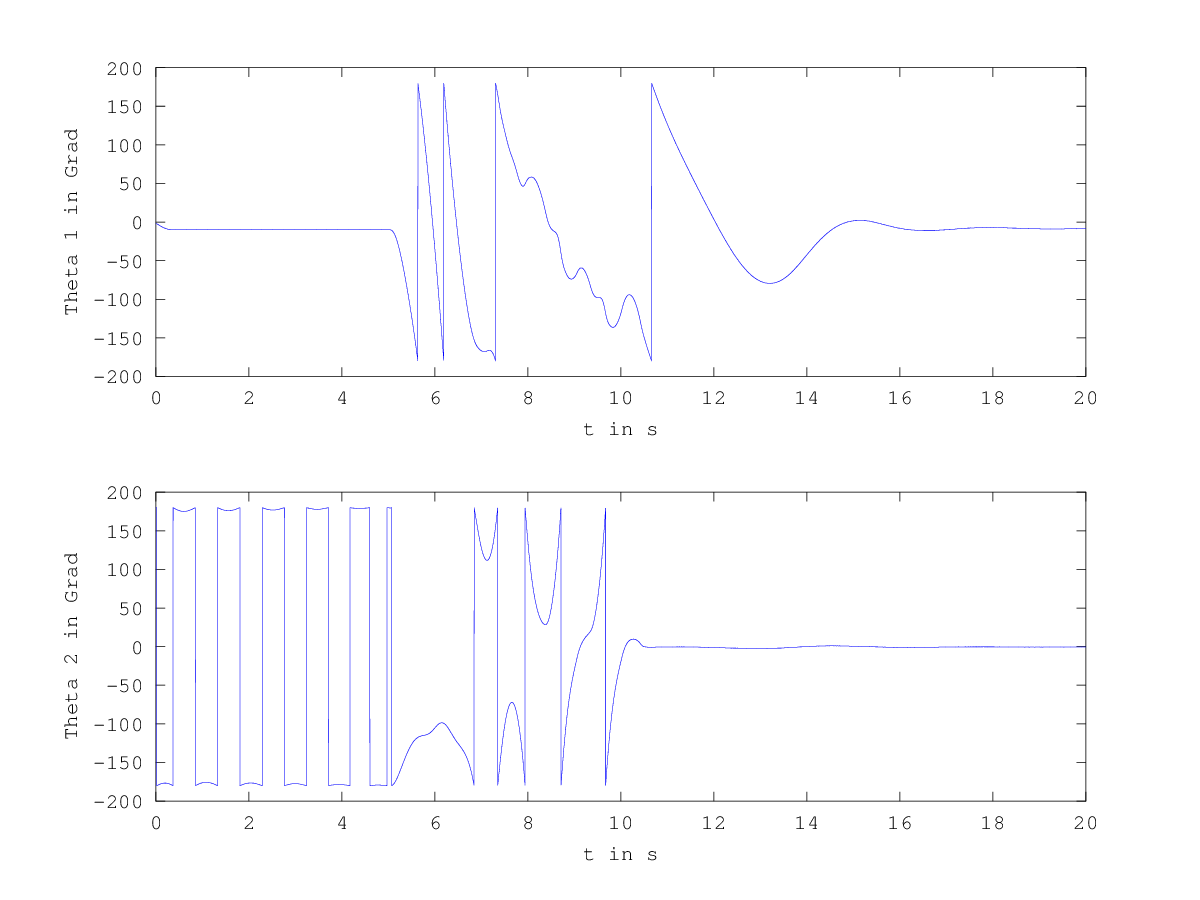
\includegraphics[width=0.8\textwidth]{Grafiken/Swingup_kurz.png}
	\caption{Initiale Pendelidentifkation}
	\label{fig.Identifikation}
\end{figure}


%\label{sec.Controller}
%\subsection{Signalverarbeitung}
%\label{signalverarbeitung} 
%Das Ausgangssignal der Inkrementalgeber wird zunächst auf Radiant-Werte umgerechnet 

\subsection{Swing-Up-Controller}
\label{Swing-Up-Controller} 

Der Swing-Up-Controller soll dem Aufschwingen des Pendels im Bereich $20^\circ < \left| \theta_2 \right| < 90^\circ$ dienen und basiert auf der Lyapunov-Funktion. Diese führt dazu, dass sich bei der Wahl von
$ \theta_2 = 0$ in der aufrechten Position des Pendels ein Regler ergibt, welcher die Energie des Pendels minimiert:

\begin{equation}
U_{SU} = n \cdot g \cdot sign(E-E_0)\dot{\theta}_2\cos(\theta_2)
\end{equation}

Der Term $E_0$ beschreibt die gewünschte, minimale Energie des Systems. Die Energie des Pendels $E$ setzt sich aus der potentiellen Energie $E_{pot}$ und der kinetischen Energie $E_{kin}$ zusammen. Die potentielle Energie lässt sich aufgrund der Referenz im höchsten Punkt des Pendels wie folgt berechnen:
\begin{equation}
E_{pot} = m_2 \cdot g \cdot l_2 \cdot (cos(\theta_2)-1)
\end{equation}

Die kinetische Energie ergibt sich zu:

\begin{equation}
E_{kin} = \frac{J_0}{2} \cdot \dot{\theta_2}^2
\end{equation}

Die Umsetzung des Reglers in Simulink ist in Abbildung \ref{fig.Simu_Swing-Up} zu sehen. 

\begin{figure}[h!]
  \centering	
  	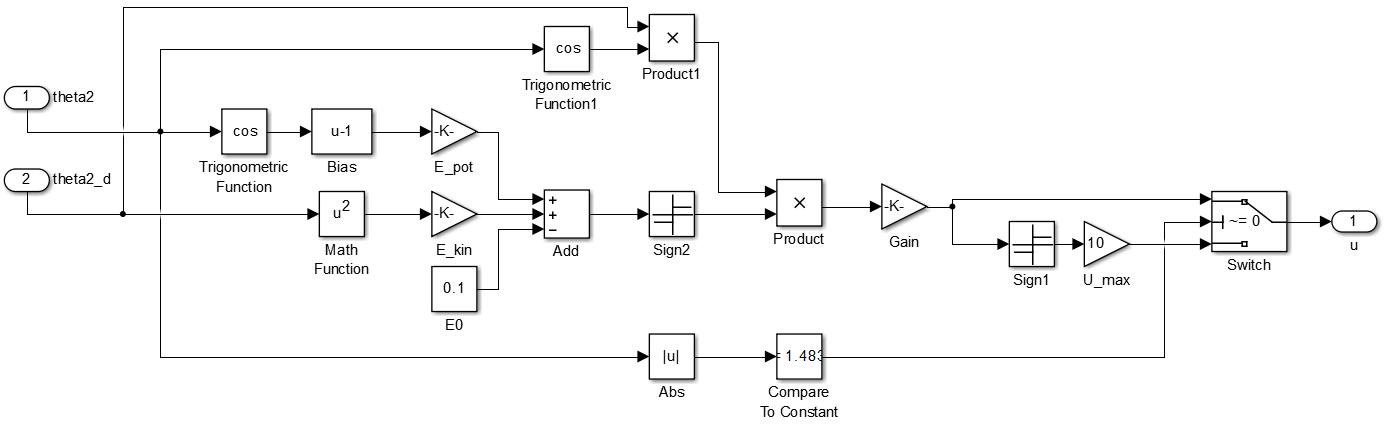
\includegraphics[width=1\textwidth]{Grafiken/simulink_swingup.png}
      \caption{Swing-Up-Controller und Zweipunktregler}
	\label{fig.Simu_Swing-Up}
\end{figure}


\subsection{Zweipunktregler}
\label{zweipunktregler} 

Für den Bereich $\left| \theta_2 \right| \geq 90^\circ$ soll ein Zweipunktregler (eng. Bang-bang control) das invertierte Pendel regeln. Dieser schaltet die maximale positive oder negative Spannung auf den Motor, abhängig von $ \theta_2 $ und $ \dot{\theta_2} $, daraus folgt die Übertragungsfunktion:

\begin{equation}
U = 10 \cdot sign(U_{SU} \cdot \theta_2 \cdot \cos(\dot{\theta}_2))
\end{equation}

Die Implementierung in Simulink ist ebenfalls als Teil des Modells in Abbildung~\ref{fig.Simu_Swing-Up} zu erkennen (Signum- und Gain-Baustein zusätzlich zum Swing-Up-Controller).


\subsection{Catcher}
\label{catcher} 

Der Catcher dient der genaueren Regelung des Pendels nahe des oberen Equilibriums von $ \theta_2 $. Um in dem Bereich optimal und robust zu Regeln, wird ein LQ-Regler verwendet. Dieser basiert auf der Minimiering der Cost-Function, welche folgenden Form besitzt:

\begin{equation}
 V = \int_0^\infty \! (x^T(t) Qx(t) + u^t(t) R u(t))  \mathrm{d}t
\end{equation}

Erhöht man die Diagonalwerte der Q-Matrix, werden die Fehler stärker Gewichtet, allerdings steigt auch der Aufwand der Regelung. Die Matrix lässt sich über die Controllability-Matrix $C$ und den linken Eigenvektor q der Matrix $A$
wie folgt berechnen:

\begin{equation}
 Q = C' \cdot q'^T \cdot q^T \cdot C
\end{equation}

Für den Vektor $q$ wurden folgenden Werte angenommen:

\begin{equation}
q =\begin{bmatrix}
         180/\pi/180 \\
         0\\
         0\\
         180/\pi/0.1
        \end{bmatrix}
\end{equation}
 
Die Diagonalwerte der Matrix R der Cost-Funktion beeinflussen die Geschwindigkeit der Regelung und wurden zunächst für den Catcher auf~$1$ gesetzt.
Zusammen mit den Eingangs- und Ausgangsmatrizen A und B lässt sich mithilfe des Matlab-Befehls $F = -lqr(A,B,Q,R)$ der LQR-Controller generieren.\citep{Werner.2013}

Die L-Matrix lässt sich über die Riccati-Gleichung herleiten, siehe \citep{Werner.2013}. Zunächst ergibt sich die P-Matrix als Lösung der Ricatti-Gleichung, daraus lässt sich mithilfe der bekannten Matritzen und des Place-Befehls $L=-place(A',C',p)'$ in Matlab berechnen.
Das Simulink-Modell des Observers ist in Abb. \ref{fig.obs_catcher} zu sehen.

\begin{figure}[htbp]
	\centering	
	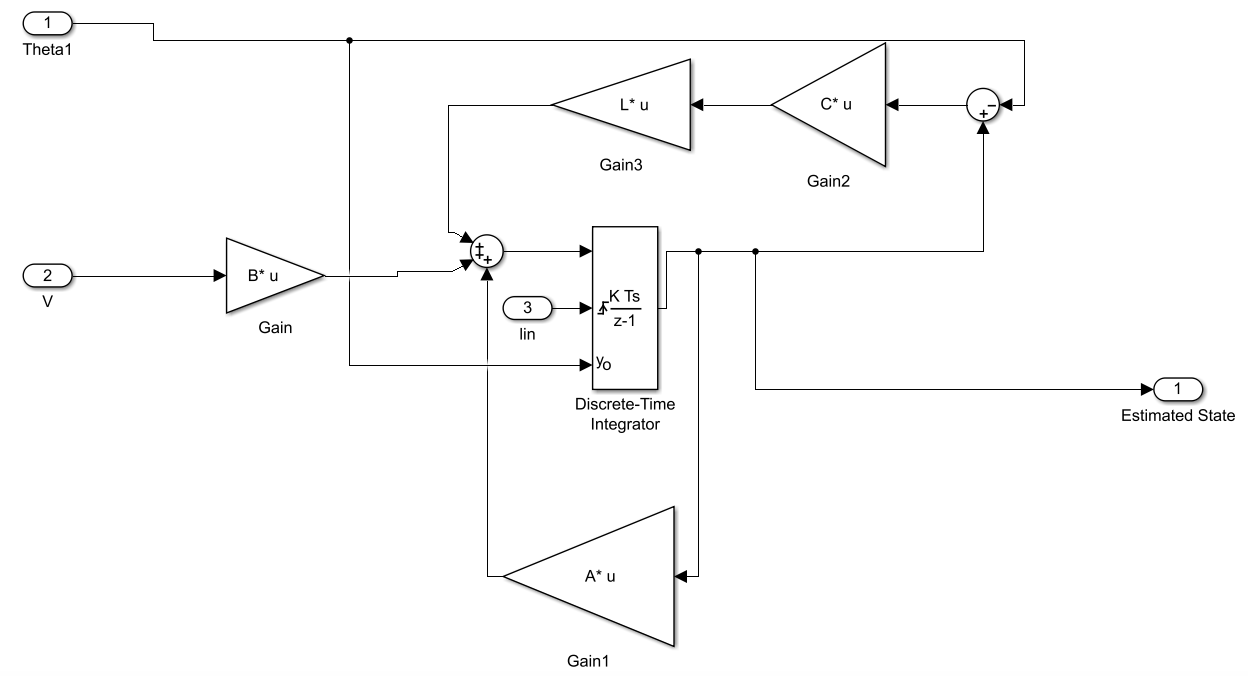
\includegraphics[width=0.8\textwidth]{Grafiken/simulink_observer_catcher.png}
	\caption{Observer des Catchers in Simulink}
	\label{fig.obs_catcher}
\end{figure}

\subsection{Stabilizer}
\label{stabilizer} 

Zur Rückführung des Pendels auf die Ausgangswinkel von $\theta_1$ und Beibehaltung der oberen Equilibrium-Position wird auch eine LQ-Regelung verwendet, welche sich nur durch die dreifache Einheitsmatrix für R und folgenden q-Vektor von dem Catcher unterscheidet:

\begin{equation}
q =\begin{bmatrix}
         180/\pi/1 \\
         0\\
         0\\
         180/\pi/0.1
        \end{bmatrix}
\end{equation}

Der Observer des Stabilizers ist in Abbildung \ref{fig.obs_stabilizer} dargestellt, während Abbildung \ref{fig.top_equilibrium} einen Überblick über die Verschaltung des Catchers und Stabilizers bietet.

\begin{figure}[htbp]
	\centering	
	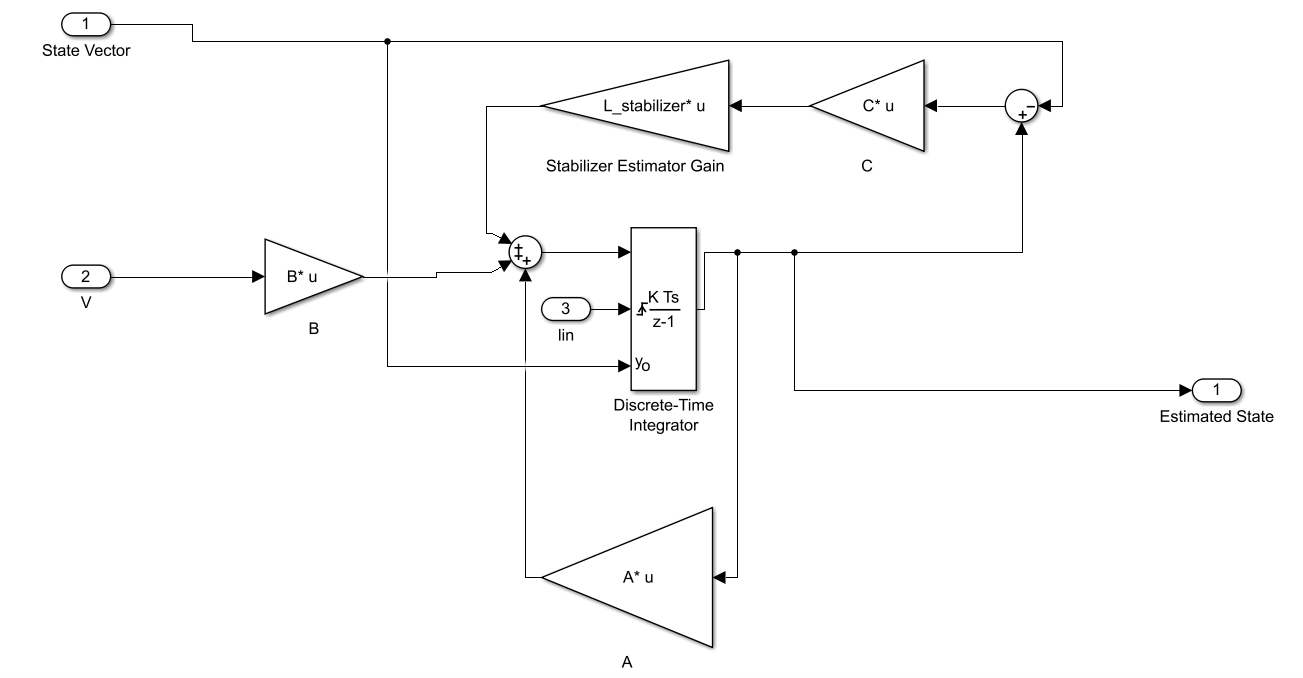
\includegraphics[width=1\textwidth]{Grafiken/simulink_observer_stabilizer.png}
	\caption{Simulink-Block des Observers des Stabilizers}
	\label{fig.obs_stabilizer}
\end{figure}

\begin{figure}[h!]
	\centering	
	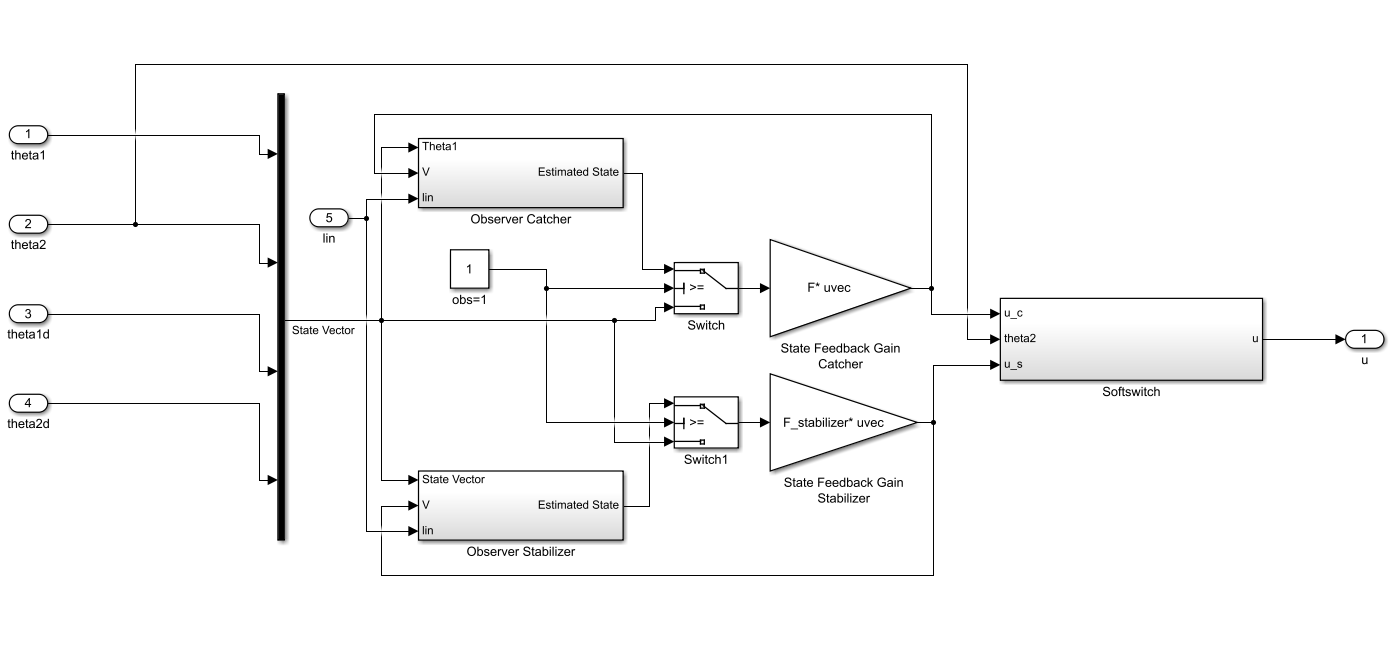
\includegraphics[width=1\textwidth]{Grafiken/simulink_top_equilibrium.png}
	\caption{Aufbau des Catchers und Stabilizers in Simulink}
	\label{fig.top_equilibrium}
\end{figure}

\subsection{Soft-Switch}
\label{Softswitch}
Um den Übergang zwischen dem Catcher und dem stabilisierenden Controller möglichst weich zu gestalten, wurde ein Soft-Switch implementiert.

Ziel dieses Switches ist es, extreme Sprünge des Controllerausgangssignals beim Umschalten zwischen den Controllern zu verhindern, selbst wenn die einzelnen Regelsignale des Catchers und des Stabilizers sehr weit auseinander liegen.

\begin{figure}[htbp]
	\centering	
	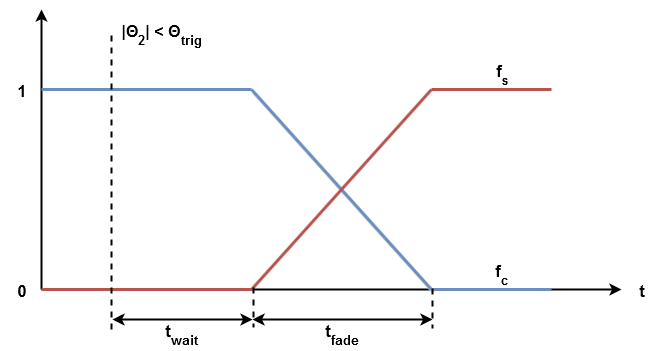
\includegraphics[width=0.8\textwidth]{Grafiken/SoftSwitch.png}
	\caption{Soft-Switch}
	\label{fig.Soft-Switch}
\end{figure}

Die Umsetzung erfolgt, indem die einzelnen Regelsignale mit Verstärkungsfaktoren multipliziert werden, die in der Summe genau~$1$ ergeben, und sich das Gesamtsignal aus den gewichteten Einzelsignalen zusammensetzt.

Zunächst ist lediglich der Catcher aktiv. Dies kommt dadurch zum Ausdruck, dass sein Verstärkungsfaktor $f_c$ den Wert 1 besitzt. Folglich muss der Faktor $f_s$ des Stabilizers 0 betragen.

Wenn nun der Betrag des Winkels $\theta_2$ für mindestens $t_{wait}$ kleiner als $\theta_{trig}$ ist, beginnt der Crossfader, das Verhältnis der Regelsignale zu verändern.
Während der Faktor des Catchers innerhalb der Zeit $t_{fade}$ linear von 1 auf 0 abfällt, erhöht sich der Faktor des Stabilizers gegenläufig innerhalb derselben Zeit von 0 auf 1.
Nach Abschluss dieses Vorgangs ist nur noch der Stabilizer für die Regelung des Pendels zuständig (vgl. Abbildung \ref{fig.Soft-Switch}). \\

Wird zu irgendeiner Zeit der Winkel $\theta_{trig}$ überschritten, wird augenblicklich mittels eines Hard-Switches der Catcher wieder aktiv geschaltet.

In unserem Controller wurden die Werte wie folgt gewählt:
\begin{eqnarray*}
&& \theta_{trig} = 5^{\circ} \\
&& t_{wait} = 0.5 s \\
&& t_{fade} = 5 s
\end{eqnarray*}

\begin{figure}[htbp]
	\centering	
	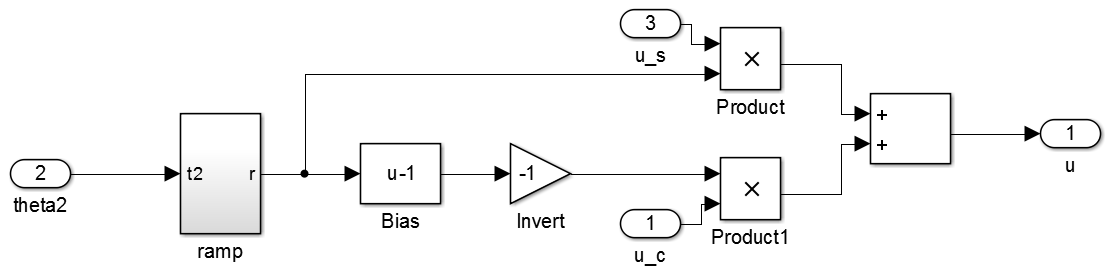
\includegraphics[width=0.8\textwidth]{Grafiken/simulink_softswitch.png}
	\caption{Soft-Switch in Simulink}
	\label{fig.Simu_Soft-Switch}
\end{figure}

Die Abbildung~\ref{fig.Simu_Soft-Switch} zeigt die Umsetzung dieses Soft-Switches in Simulink. Der Block `ramp' erzeugt dabei den Faktor $f_s$ woraus sich ebenfalls $f_c$ ableiten lässt.

Als Timer, wie sie innerhalb des `ramp' - Blocks zu finden sind, werden grund\-sätz\-lich Integrator-Blöcke verwendet. Schließt man am Eingang eines solchen Integrators die Konstante $1$ an, so ist der Wert des Ausgangs die Zeit seit dem letzten Reset.\\

\textit{Hinweis:} Die Funktionsweise dieses Verfahrens ist dabei identisch mit der eines Crossfaders, wie er teilweise beim Übergang zwischen zwei Musikstücken verwendet wird.


%----------------------------------------------------------------------------------------
%	SECTION 5
%----------------------------------------------------------------------------------------
\section{Ergebnisse}
In diesem Kapitel sind Versuchsergebnisse dargestellt, die an dem geregelten Pendel gewonnen wurden. Dafür wurde das stabilisierte Pendel mit einem kurzen Störimpuls beaufschlagt und die Reaktion aufgezeichnet. Dieser Störimpuls erfolgte per Hand und wurde in unterschiedlichen Stärken durchgeführt, um so die einzelnen Controller testen zu können. 
\subsection{Swing-Up}
Zunächst soll anhand von Abbildung \ref{fig.Swing-Up-Plot} der Aufschwing-Vorgang betrachtet werden. Wie bereits in Kapitel \ref{Pendelidentifikation} erwähnt, vollzieht der Controller in den ersten 5 Sekunden die Identifikation des Pendels. Der dafür verwendete Impuls lässt sich bei $\theta_1$ nahe $t=0s$ erkennen. Nach diesen 5 Sekunden beginnt der Controller zunächst durch Verwendung des Zweipunktreglers und des Swing-Ups den Pendelarm in den Bereich $\left| \theta_2 \right| < 20^\circ$ zu bewegen, in welchem dann der Catcher aktiv wird, um ein Überschwingen zu verhindern. Nach einer kurzer Zeit, in der gilt $\left| \theta_2 \right| < 5^\circ$, übernimmt dann der Stabilizer mehr und mehr die Kontrolle (vgl. Kapitel \ref{Softswitch}), welcher schließlich auch $\theta_1$ auf seinen Anfangswinkel regelt.

\begin{figure}[htbp]
	\centering
	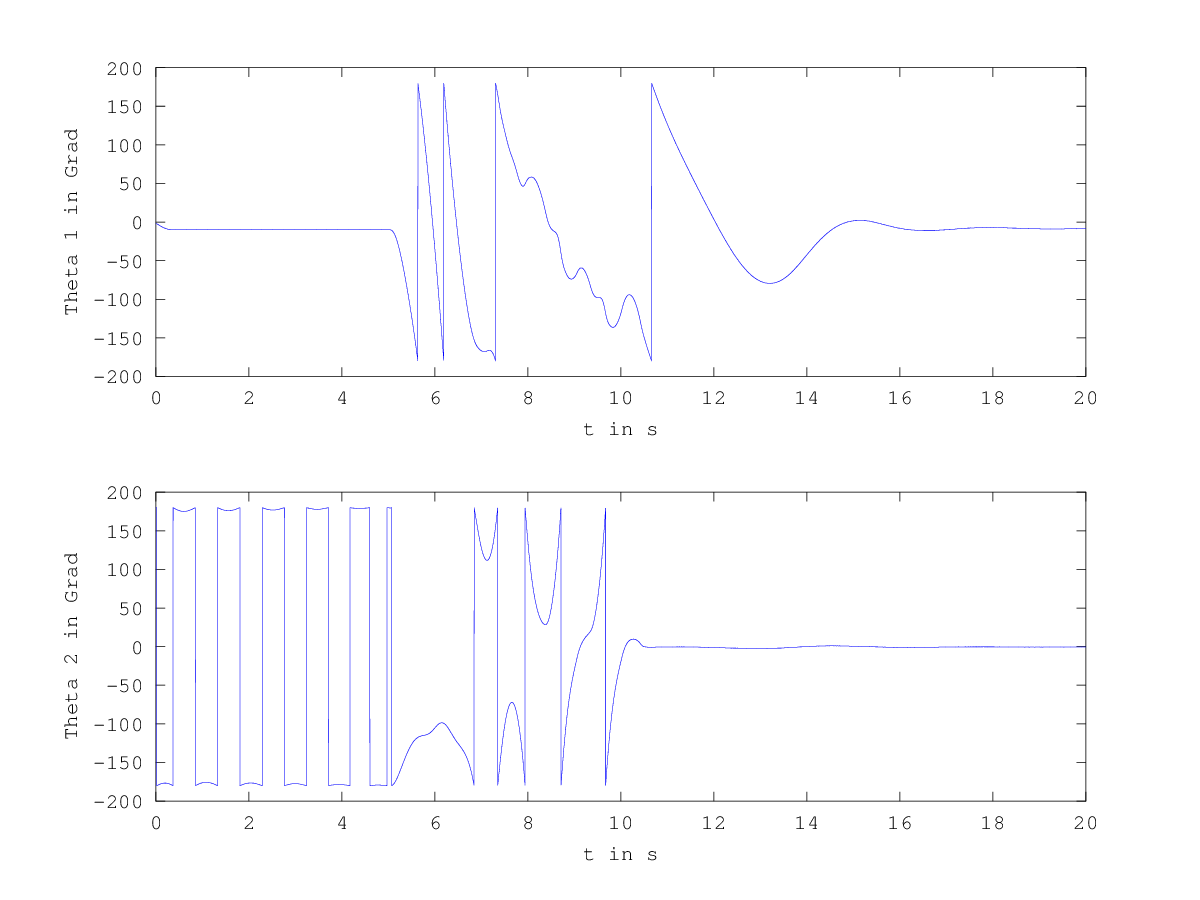
\includegraphics[width=1.\textwidth]{Grafiken/Swingup_kurz.png}
	\caption{Der Swing-Up-Vorgang}
	\label{fig.Swing-Up-Plot}
\end{figure}


\subsection{Stabilisierer}

<<<<<<< HEAD
Der Stabilisierer wird in Abb. \ref{fig.Stabilisierer-Plot} durch eine schwachen Impuls getestet, wodurch $\theta_2$ um 2 Grad ausgelenkt wurde. Dadurch bleib der Stabilizer weiterhin aktiv und regelt die Motorspannung so, dass über das Überschwingen von $ \theta_1$ das Pendel wieder in die obere Position gebracht wird. Zudem ist auch zu erkennen, dass der Regler auch $ \theta_1$ in die Ausgangsposition zurückführt.
=======
Der Stabilisierer wird in Abb. \ref{fig.Stabilisierer-Plot} durch eine schwachen Impuls getestet, wodurch $\theta_2$ um 2 Grad ausgelenkt wurde. Dadurch bleibt der Stabilizer weiterhin aktiv und regelt die Motorspannung so, dass über das Überschwingen von $ \theta_1$ das Pendel wieder in die obere Position gebracht wird. Zudem ist zu erkennen, dass der Regler auch hier $ \theta_1$ in die Ausgangsposition zurückführt.

>>>>>>> master
\begin{figure}[htbp]
	\centering
	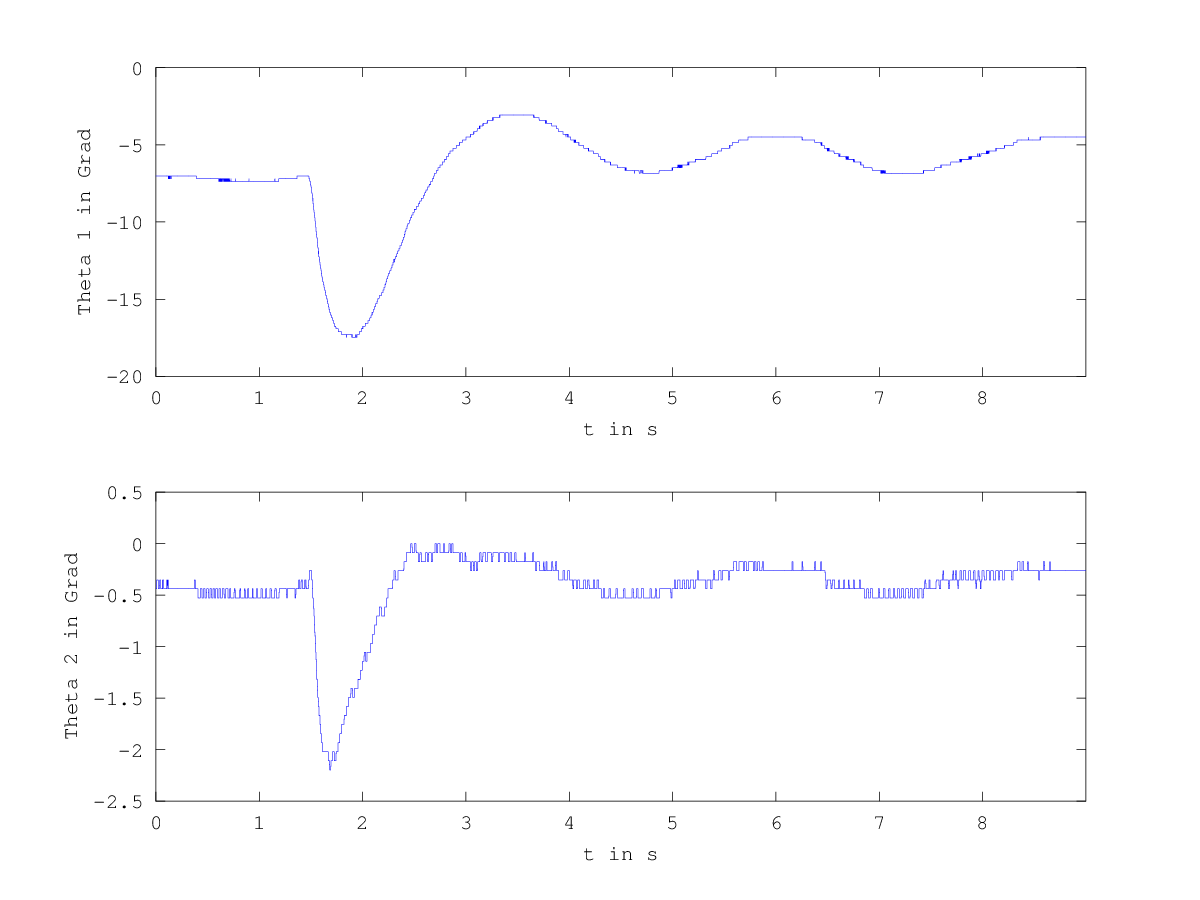
\includegraphics[width=1.\textwidth]{Grafiken/Stab_lang.png}
	\caption{Störung \textless $5^{\circ}$}
	\label{fig.Stabilisierer-Plot}
\end{figure}


\subsection{Catcher}
In Abb. \ref{fig.Catcher-Plot} sind die Auswirkungen des Reglers nach einer Störung von 9 Grad zu erkennen. Der Catcher sorgt dabei zunächst für ein schnelles Rückstellen des Pendels auf das Top Equilibrium, während nach der 3. Sekunde der Einfluss des Stabilizers steigt und dieser im Mittel $\theta_1$ gegen 0 Grad regelt, allerdings mit starken Schwingungen, um die Abweichung von $\theta_2$ auszugleichen. 
\begin{figure}[htbp]
	\centering
	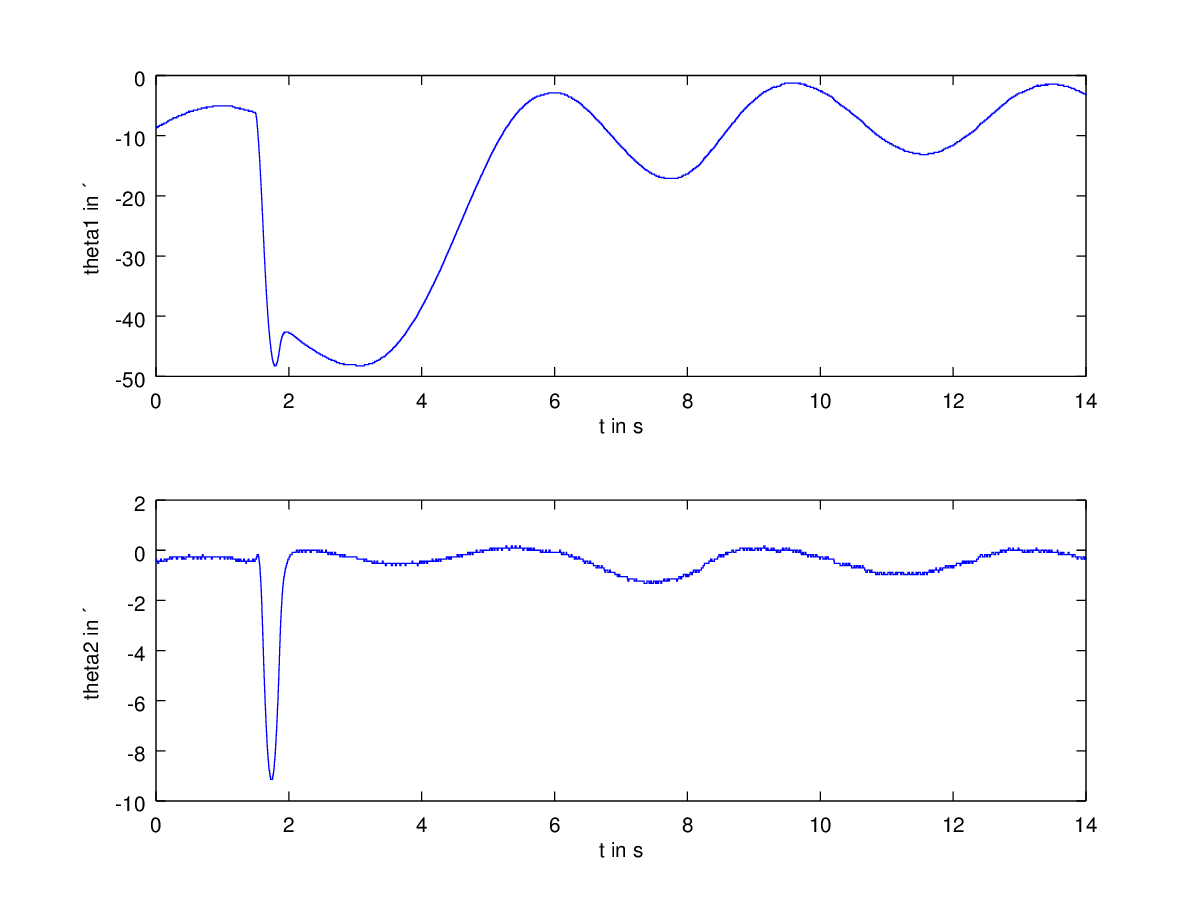
\includegraphics[width=1.\textwidth]{Grafiken/Catch_kurz.png}
	\caption{Störung \textgreater $5^{\circ}$}
	\label{fig.Catcher-Plot}
\end{figure}

\subsection{Watchdog}
Hin und wieder kommte es vor, dass das System in einen Zustand gerät, in dem es das Pendel nicht mehr fangen und in das Top Equilibrium zurückbringen kann. Dieser Zustand in in Abbildung \ref{fig.Watchdog-Plot} zu sehen. Um ein solches Verhalten zu verhindern, könnte man einen Watchdog implementieren, der anhand der Winkelgeschwindigkeit $\dot{\theta}_1$ erkennt, wenn das Pendel nicht mehr erfolgreich geregelt werden kann. Liegt der Wert von $\dot{\theta}_1$ für eine bestimmte Zeit nicht in dem Intervall $[-\epsilon,+\epsilon]$, so kann der Watchdog einen kurzzeitigen Stopp des Pendels veranlassen und es anschließend neu starten.

\begin{figure}[htbp]
	\centering
	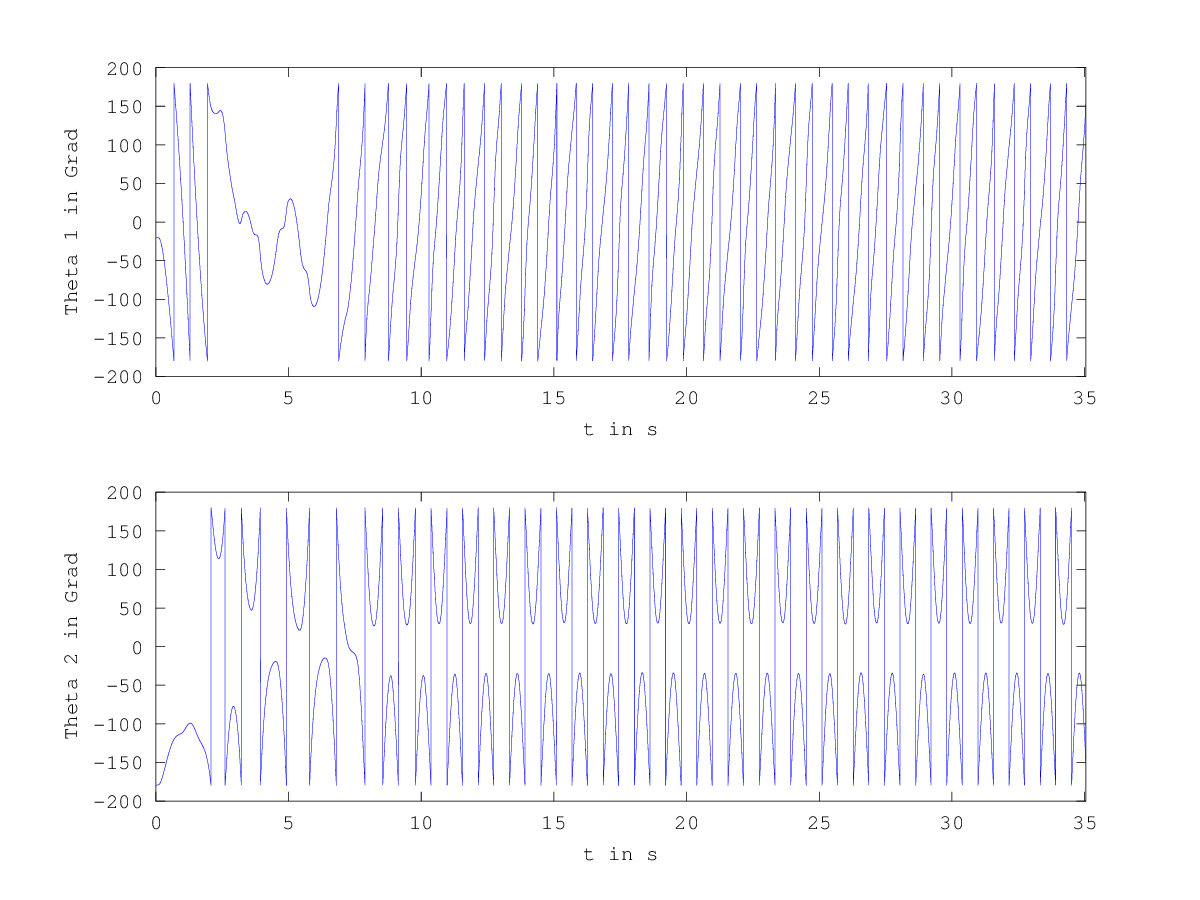
\includegraphics[width=1.\textwidth]{Grafiken/Watchdog_lang.png}
	\caption{Watchdog}
<<<<<<< HEAD
\end{figure}\section{Ergebnisse}
=======
	\label{fig.Watchdog-Plot}
\end{figure}


>>>>>>> master


%----------------------------------------------------------------------------------------
%	Ursprünglicher Inhalt dieses Dokuments
%----------------------------------------------------------------------------------------
%\section{Experimental Data}

\begin{tabular}{ll}
Mass of empty crucible & \SI{7.28}{\gram}\\
Mass of crucible and magnesium before heating & \SI{8.59}{\gram}\\
Mass of crucible and magnesium oxide after heating & \SI{9.46}{\gram}\\
Balance used & \#4\\
Magnesium from sample bottle & \#1
\end{tabular}

%----------------------------------------------------------------------------------------
%	SECTION 3
%----------------------------------------------------------------------------------------

\section{Sample Calculation}

\begin{tabular}{ll}
Mass of magnesium metal & = \SI{8.59}{\gram} - \SI{7.28}{\gram}\\
& = \SI{1.31}{\gram}\\
Mass of magnesium oxide & = \SI{9.46}{\gram} - \SI{7.28}{\gram}\\
& = \SI{2.18}{\gram}\\
Mass of oxygen & = \SI{2.18}{\gram} - \SI{1.31}{\gram}\\
& = \SI{0.87}{\gram}
\end{tabular}

Because of this reaction, the required ratio is the atomic weight of magnesium: \SI{16.00}{\gram} of oxygen as experimental mass of Mg: experimental mass of oxygen or $\frac{x}{1.31}=\frac{16}{0.87}$ from which, $M_{Mg} = 16.00 \times \frac{1.31}{0.87} = 24.1 = \SI{24}{\gram\per\mole}$ (to two significant figures).

%----------------------------------------------------------------------------------------
%	SECTION 4
%----------------------------------------------------------------------------------------

\section{Results and Conclusions}

The atomic weight of magnesium is concluded to be \SI{24}{\gram\per\mol}, as determined by the stoichiometry of its chemical combination with oxygen. This result is in agreement with the accepted value.

\begin{figure}[h]
\begin{center}
%\includegraphics[width=0.65\textwidth]{placeholder} % Include the image placeholder.png
\caption{Figure caption.}
\end{center}
\end{figure}

%----------------------------------------------------------------------------------------
%	SECTION 5
%----------------------------------------------------------------------------------------

\section{Discussion of Experimental Uncertainty}

The accepted value (periodic table) is \SI{24.3}{\gram\per\mole} \cite{Smith:2012qr}. The percentage discrepancy between the accepted value and the result obtained here is 1.3\%. Because only a single measurement was made, it is not possible to calculate an estimated standard deviation.

The most obvious source of experimental uncertainty is the limited precision of the balance. Other potential sources of experimental uncertainty are: the reaction might not be complete; if not enough time was allowed for total oxidation, less than complete oxidation of the magnesium might have, in part, reacted with nitrogen in the air (incorrect reaction); the magnesium oxide might have absorbed water from the air, and thus weigh ``too much." Because the result obtained is close to the accepted value it is possible that some of these experimental uncertainties have fortuitously cancelled one another.

%----------------------------------------------------------------------------------------
%	SECTION 6
%----------------------------------------------------------------------------------------

\section{Answers to Definitions}

\begin{enumerate}
\begin{item}
The \emph{atomic weight of an element} is the relative weight of one of its atoms compared to C-12 with a weight of 12.0000000$\ldots$, hydrogen with a weight of 1.008, to oxygen with a weight of 16.00. Atomic weight is also the average weight of all the atoms of that element as they occur in nature.
\end{item}
\begin{item}
The \emph{units of atomic weight} are two-fold, with an identical numerical value. They are g/mole of atoms (or just g/mol) or amu/atom.
\end{item}
\begin{item}
\emph{Percentage discrepancy} between an accepted (literature) value and an experimental value is
\begin{equation*}
\frac{\mathrm{experimental\;result} - \mathrm{accepted\;result}}{\mathrm{accepted\;result}}
\end{equation*}
\end{item}
\end{enumerate}
%----------------------------------------------------------------------------------------
%	BIBLIOGRAPHY
%----------------------------------------------------------------------------------------

\bibliographystyle{apalike}

\bibliography{Kapitel/report-bib}

%----------------------------------------------------------------------------------------


\end{document}